\chapter{MAC Protocols}\label{sec:protocols}
\section{Considerations}\label{sec:mac_considerations}
\ac{phy} testing indicated that \ac{lora} is suitable for single-hops in a system with sparsely separated radios; ranges of 500m can be expected for $\text{\ac{sf}}=11$ (\ac{dr}1) regardless of the propagation environment. However, even with the 1600m range offered in free space, single-hop point-to-point coverage to all radios is unlikely, leading to the expected dynamic mesh topology.

With this in mind, three contention-based \ac{mac} protocols are considered to handle the requirement of data transfers to physically close neighbours: a base case (ALOHA), a common approach (\ac{csma}) and a scenario specific approach (\ac{llbp}). Attempting to make as many radios as possible receive a transmission is of little help; if local-interest data is received 1500m away, from the receiver's perspective the transmission is unwanted and increasing the chance of a local collision. To this end a wanted criteria is defined as the maximum distance for which data is considered helpful; this is set to the worst-case minimum transmission distance (500m).

The \ac{lora} configurations considered for use are the abstracted \ac{dr}s from \ac{lorawan} \cite{3YP:LORAWAN_REGIONAL_PARAMS}; however, DR0 and DR2 are disregarded due to their lack of respective \ac{sf} performance. Although small packets ($< 20\enskip \text{bytes}$) have been shown to have slightly higher receive probability, they are not practical with transmission overhead, therefore packets are allowed to be any size ($< 255\enskip \text{byte limit}$). 

As opposed to the \ac{lorawan} \ac{dc} manager (see Figure \ref{fig:lorawan_duty_cycles}), all protocols use a custom \ac{dc} manager proposed in Appendix \ref{sec:proposed_duty_cycle}. This is  more flexible because it considers airtime over the full enforcement interval ($d_i$), allowing multiple sequential transmissions without silence; this is a requirement for bulk transmissions or protocol handshakes. The simulator provides support for both models.
\section{Approaches}


\subsection{ALOHA}
Uses \ac{lorawan}'s principle of just sending data periodically provided the \ac{dc} limit allows. No channel sensing is carried out, but transmissions will be delayed if the transmitter is synchronised at the scheduled time. For purposes of testing, the minimum spacing between transmissions is that enforced by \ac{lorawan}. Therefore, in the case that any backoff occurs, less than the \ac{dc}'s maximum worth of data will be transmitted. \ac{mac} performance purely relies on each radio only using a small amount of airtime. As all radios must be on the same configuration the method can only use a single channel and \ac{dr} -- no mechanism is used for dynamically agreeing parameter changes. Consequently, a fixed \ac{dc} of up to 10\% is supported on band h1.6. Test packets use random payload sizes and all packets are treated as data, acknowledgement and retransmission overhead is not considered. \ac{tp} is assumed to be fixed to 14dBm for all scenarios.

\subsection{CSMA}
Uses the ALOHA approach but does carrier-sensing using \ac{lora}'s \ac{cad} process immediately before transmissions. On detection, random backoff will occur before the \ac{cad} process repeats; this is a simplified approach to that proposed in \cite{3YP:LORA_CSMA}. The \ac{ps} are increased from 8 to 32 to increase likelihood of preamble detection with the drawback of increased airtime overhead. When all nodes are within range of one another the vulnerable collision period is very short; provided no failed synchronisations take place, collisions should only occur if two transmitter's \ac{cad}s overlap, however collisions resulting from the hidden node problem (Figure \ref{fig:hidden_node_problem}) are not avoided. Other mentioned ALOHA limits apply.

\begin{figure}[H]
    \centering
   	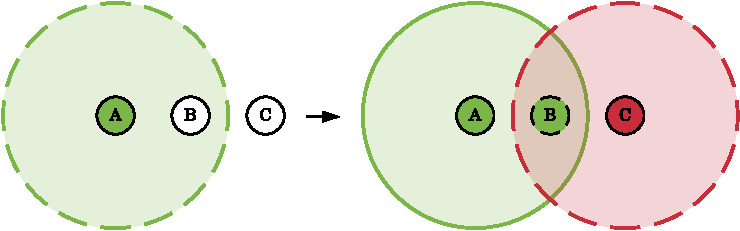
\includegraphics{Figures/hidden_node_problem}
    \caption[Demonstration of hidden node problem]{
    	Demonstration of the hidden node problem. A has transmitted before C, however, C was unable to sense A and assumes it is okay to transmit. B will likely receive no signal due to noise.
    }
    \label{fig:hidden_node_problem}
\end{figure}


\subsection{LoRa Local Broadcast Protocol (\ac{llbp})}
This is a bespoke approach that makes use of dynamic channel and \ac{sf} switching with the target of constricting receivability to local listeners. The protocol uses two bands: a management-band (h1.4) and a data-band (h1.3). The former is treated as a single \ac{csma} channel, whereas the latter allocates 15 channels at \ac{cf}s $865.1 + 0.2 \cdot C_n$ (\ac{bw}=125kHz).

In principle, the protocol announces when a transmitter has a large chunk of data to send using a data announcement packet (\ac{dap}); this contains the \ac{lora} configuration to switch to and a description of the data being sent (Figure \ref{fig:dap_packet}). When a radio receives this packet it can make its own decision on whether it wants the data; if it does not it can ignore the message and will never see any data packets, otherwise it can switch configurations and only see those packets. 

\begin{figure}[H]
    \centering
   	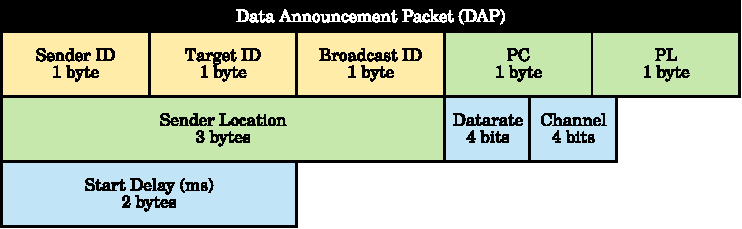
\includegraphics{Figures/dap}
    \caption[Data Announcement Packet \ac{dap}]{
    	
    }
    \label{fig:dap_packet}
\end{figure}

As opposed to agreeing the configuration with a flurry of transmissions at one point, the configuration is decided by the transmitter, using its prior knowledge of surrounding transmitters. This knowledge is gained through periodical heartbeat packets (Figure \ref{fig:heartbeat_packet}), sent on the management-band; these provide \ac{snr}s and locations. The fastest viable \ac{dr} is picked along with a random data-band channel. There is no guarantee the channel is free but with the number of available channels, and a compulsory 1\% \ac{dc} across all of them, collisions are unlikely. \ac{dr} is selected such that for wanting receivers $\min(\text{\ac{snr}}) > (D_l + 2.5)$; this is where \ac{prp} should be approximately 100\%.

\begin{figure}[H]
    \centering
   	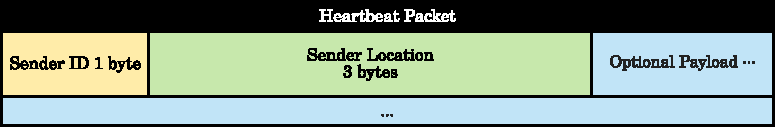
\includegraphics{Figures/heartbeat_packet}
    \caption[Heartbeat Packet]{
    	
    }
    \label{fig:heartbeat_packet}
\end{figure}

The side effect of choosing the fastest \ac{dr} is less airtime, although this could be used to achieve more throughput, instead it is used to keep interference times to a minimum for the same data. The approach is high-risk, in the event a \ac{dap} is missed, or prior knowledge is incorrect, intended recipients may not receive any data. The number of \ac{dap}s sent can be increase to reduce the probability of the first case. However, increasing heartbeat frequency for the second case is problematic as it increases the likelihood in \ac{dap}s getting missed. Heartbeats and \ac{dap}s are both considered as overhead. 
%Like with the other protocols, acknowledgements and retransmissions are not attempted.
 

\section{Test Methodology}
The simulator provides a number of environment presets. That most applicable to protocol testing, \texttt{LargeDataBroadcastTest}, provides automatic generation of an $[x \times y]$ radio grid where spacing ($S$) is the same $\pm 20\%$. It provides four obstruction options seen in Figure \ref{fig:large_broadcast_options}.


\begin{figure}[H]
    \centering
   	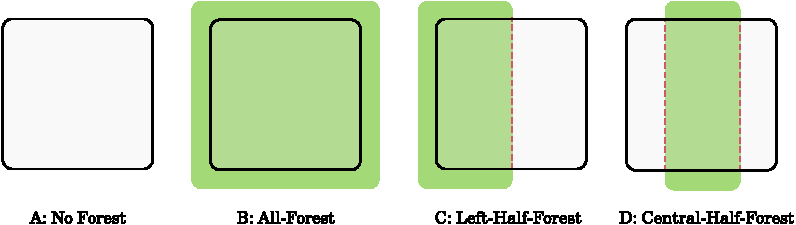
\includegraphics{Figures/test_environments}
    \caption[\texttt{LargeDataBroadcastTest} obstruction options]{
    	\texttt{LargeDataBroadcastTest} obstruction options, green indicates forest where $\beta = 0.55$. Radios are scattered in the black square
    }
    \label{fig:large_broadcast_options}
\end{figure}


% no obstructions, full-forest coverage, half-forest left-side and half-forest central, where $\beta = 0.55$ for all; see . 

If radios were always able to use their fastest configuration, it is highly unlikely a protocol with overhead would outperform one without. To alleviate this unfairness, $S$ was set to $400m$; ensuring that in-forest radios needed \ac{dr}1 to communicate, but giving other transmissions the opportunity to increase \ac{dr}. 

The protocol configurations executed for each environment were:
\vspace{-5mm}
\begin{itemize}
\item ALOHA with \ac{dc}s of 1\% \textbf{[A]} and 10\% \textbf{[B]}.
\item CSMA with \ac{dc}s of 1\% \textbf{[C]} and 10\% \textbf{[D]}.
\item LLBP with \ac{dap} count of 1 \textbf{[E]} and 2 \textbf{[F]}.
\item LLBP with \ac{dap} count of 1 where true locations and \ac{snr} values were known (perfect heartbeat information) \textbf{[G]}. 
\end{itemize}
\vspace{-5mm}
\textit{For \ac{llbp} heartbeats are sent for 50\% of the 1\% \ac{dc}.}

Each of the 28 configurations was executed in the simulator for 6 hours of simulation time, after which simulator statistics were exported.

\section{Results \& Discussion}
Approaches suited to DTN



% 1\% vs 10\% is provided to highlight the issue with high data sending
%Fundamentally \ac{llbp} only has a 1\% \ac{dc} for test data, and can only be expect throughput to that level.
%This is compared to if the heartbeat packets were not required and all radios had perfect data. This demonstrates that fundamentally the protocol appears to perform less strongly, problaby because msising one packet results in many packets getting lost.





\% of intended recipients received for each message
Reasoning for failed receive: Insufficient SNR (out of range), CRC fail (bad luck), Sync Collision/ CRC from interference

Missed == This implies the receiver was busy, busy receiving at the same time or not receivable 
No Preamble on a Wanted == This implies the SF is not adequate

The protocol 
Total helpful throughput number of bytes,  number of packets



To make effectiveness comparisons fair they are 


Verification of the protocol is to be gauged on 
% Criteria of goodness is: 
 - \% of wanted packets received
 - \% of wanted bytes received
 - Total bytes received
 - Total packets delivered
 - Number of collisions on wanted messages

\begin{figure}[H]
    \centering
   	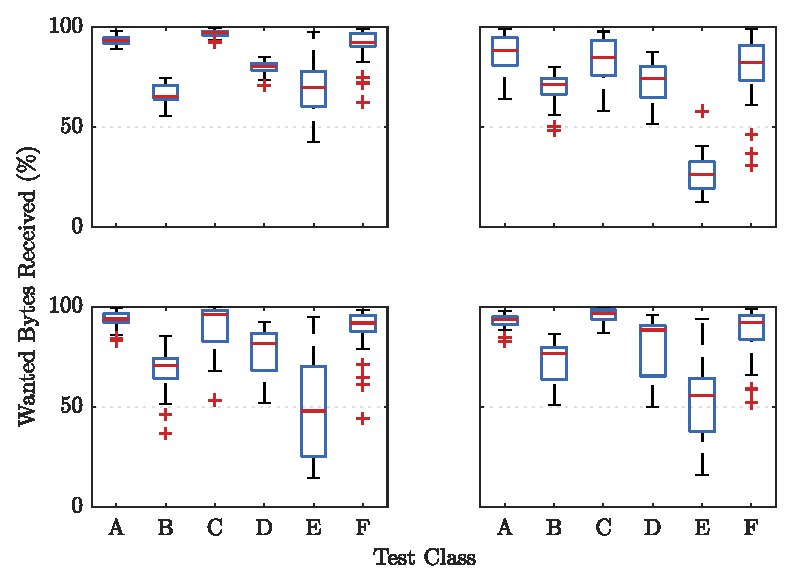
\includegraphics{Figures/sim_recv_boxplots}
    \caption[Boxplot of protocol received byte percentage]{
    	Simulat
    }
    \label{fig:sim_recv_boxplots}
\end{figure}

Optionally, an extra high-rate channel could be allocated in band h1.6 (\ac{dc}=10\%) for critical communications. However the single available channel a

%When operating at the limits of the slowest \ac{dr} there will be extra packets sent with no \ac{dr} improvement. Therefore this is likely to be a bad scenario.

%Attempting to emulate a unicast handshake into a broadcast scenario. Relying on responses to the initial transmitter requires a flurry of transmissions that do not know when others are replying causing collisions. Although the provider of the could allocate reply slots; this not only requires pin-point timing. Uses Demand Assigned Multiple Access, relies on the fact that there are many channels and low probability of getting the same band, low spreading factors keep localisation where possible, and avoid conflicts with high spreading factor long range transmissions.
%One approach may be to slot transmissions so there is always a good time to send announcements. 
%A more complex method could require a handshake between receivers and broadcaster using slotted schedules, but this is high overhead and massively increases nearby death
%If it costs more to send out the 

%This leads to the requirement of multi-hop communications and handling of the significant challenges they present, namely: collisions (Section \ref{sec:lora_considerations}) in the presence of the hidden node problem (highlighted in Figure \ref{fig:collisions}) and routing (Section \ref{sec:adhocnetworks}). 


%First check band that you're going to send in
%Use knowledge of who is around from regular broadcasts on 1 band
%Send out broadcast with slots for people to reply with CTR on other band (clear to receive)
%Send out ATT (about to transmit)
%Switch to lower sf and other band

%Unable to exploit use of spreading factors as agreement must be made to change settings globally

%Unfortunately, CA does not effectively avoid all collisions in a multi-hop network. In the first place it is not usable when broadcasting, and so it cannot be used, for example, to improve traditional flooding broadcasting. In addition, the interference range of a node is usually greater than its trans- mission range. Specifically, a radio receiver can only decode a signal if the signal power exceeds a minimum threshold, and if the signal power is at least a given factor greater than the noise or interference power. Assume an intended receiver sends a CTS to ask all its neighbors to remain quiet during the upcoming transmission. A node that is just out of range of this receiver does not decode it, and is unaware that a transmission is in progress, and so proceeds to transmit its own packet. Although the node is too distant to directly communicate with the receiver, the strength of its trans- mission (which is noise to the receiver, which is listening to a different packet) may reduce the signal-to-noise ratio at the receiver enough that the receiver is unable to decode its incoming packet. Although it is a matter of semantics whether this should be classified as interference or collision, it is clear that even for unicast transmission CA does not always prevent one node’s communication from interfering with communication among other nodes.

%Better to keep low \ac{dc}, 10\% will have massive collisions
%From PHY testing it is known that 
%Also know that if devics are moving, LOS changes in forests may suddenly cause packet failure, better to shove all data asap
